% SECTION 16: Errors in Lattice Results
% Source: extract/sec16.txt (PDF pages 98-107), from the "16. Errors in Lattice
% Results" heading to the end of the extract. The extract ends mid-sentence
% ("...extrapolate keeping only the terms in"); the closing sentence and the
% final paragraph of Section 16 (which fall at the top of extract/sec17.txt,
% PDF page 108) are completed from the author's original source
% (chap-errors.tex) so the chapter is complete.

\chapter{Errors in Lattice Results}

Numerical simulations of lattice QCD introduce both statistical and a number of systematic errors. I have collected together a brief description of the various errors here, and in the remainder of the article I will only give quantitative estimates. I will label a particular systematic uncertainty as negligible/important if it is negligible/comparable in magnitude to the statistical error for that observable as determined in a state-of-the-art calculation.

\section{Statistical errors}

The monte carlo method for doing the functional integral employs statistical sampling. The results, therefore, have statistical errors. The current understanding, based on agreement of results from ensembles generated using different update algorithms, different initial starting configuration, and different random number generators in the Markov process, is that the functional integral for QQCD is dominated by a single region. Second, we find that configurations with non-trivial topology are properly represented in an ensemble generated using a Markov chain based on small changes to link variables. Based on these observations we conclude that the energy landscape is simple, consequently, the statistical errors should fall as $1/\sqrt{N}$, where $N$ is the number of independent measurements. Tests like binning of the data and the calculation of auto-correlation times for various observables are used to determine the monte-carlo time between independent configurations.

Estimates of decorrrelation times in dynamical simulations are just becoming available and the understanding of decorrelation times for various update algorithms and different fermion formulations is not complete. A recent study of decorrelations for update of Wilson fermions [142] using the hybrid Monte Carlo algorithm [141] (the algorithm of choice) presented very encouraging results. They found that decorrelation time based on tunneling rate between different topological sectors (expected to be amongst the slowest modes) was within a factor of two of standard probes like large Wilson loops and hadron correlators, and $\approx 80$ units of molecular dynamics time for $m_\pi / M_\rho \ge 0.56$. Thus trajectory lengths of 5000--10000 units, which are feasible on todays computers, provide a reasonable statistical sample. Even though details like how this decorrelation time grows with decreasing quark mass still need to be filled in, it is clear that current Monte Carlo algorithms do provide a reliable way of doing the functional integral for both QQCD and full QCD.

\section{Finite Volume}

This is the simplest error to visualize as it is associated with using finite lattices to represent an infinite system. L\"uscher has shown that for sufficiently large lattices of side $L$, the finite volume corrections in the mass $M$ of a given state fall off as $e^{-ML}$ [27]. This anaylsis assumes that the interactions with the mirror states on a periodic lattice are small. On small lattices the wave-function of the states is squeezed, resulting in an much more rapid increase of the mass with decreasing lattice size. This effect is seen clearly for $L < 1.5$ fermi, where the finite size behavior fits a power-law, $\sim 1/L^3$ [143]. The goal, therefore, is to work on lattices large enough such that the finite size effects are exponentially suppressed.

To determine the lattice size needed for observables involving quark propagation I choose the pion as the test state as it the lightest and thus has the largest correlation length. Results of quenched simulations show that for $M_\pi L \ge 5$ the exponential suppression applies and the corrections are negligible. For physical value of $M_\pi$ this translates into $L \ge 7$ fermi. Another way of stating the same criteria is that the quantum mechanical properties of hadrons, typically of size $\le 1$ fermi, are unaltered if the box size is larger than $7$ fermi. Current simulations explore quark masses in the range $m_q \ge m_s/4$ or equivalently $M_\pi / M_\rho \ge 0.4$. For these ``heavier masses'' the criteria $M_\pi L \ge 5$ translates into $L \ge 3$ fermi. The lattices used in the most recent calculations, for example the CP-PACS runs, discussed later, satisfy this condition.

Another consequence of finite $L$ is momentum resolution. For example, the lowest non-zero momentum, and spacing, is $2\pi/La = 393$ MeV for $L = 32$ and $1/a = 2$ GeV. One would like a much finer resolution when investigating the dispersion relation for mesons and baryons or when calculating matrix elements required to study form-factors in semi-leptonic and rare decays. This can only be done by increasing either $L$ or $a$. Increasing $L$ is limited by computer resources, while increasing $a$ increases discretization errors which are discussed next.

\section{Finite lattice spacing errors}

The lattice is merely a technical scaffold and the physical results are obtained by taking the $a \to 0$ limit. At finite $a$, lattice results have discretization errors whose size depend on the degree to which the lattice action and operators have been improved (see Sections 8, 12, and 13). As discussed in Section 8, we employ two strategies for removing these errors. First, improve the lattice action and operators so that the errors at fixed $a$ are small, and secondly, repeat the simulations at a number of values of $a$ and extrapolate to $a = 0$. Since the functional form used to characterize the errors is usually truncated to just the leading term in $a$, the extrapolation has an associated systematic error. To get a handle on this uncertainty, extrapolations have been done for three different formulations (Wilson, clover, staggered) for which the leading corrections are different ($O(a)$, $O(\alpha a) - O(a^2)$, $O(a^2)$). The difference between the three results in the $a = 0$ limit is a measure of the residual uncertainty. I shall illustrate this procedure for controlling the discretization errors in Section 20 where the calculation of quark masses is discussed.

\section{Chiral Extrapolations in the light quark masses}

The physical $u$ and $d$ quark masses are too light to simulate on current lattices. For $1/a = 2$ GeV, realistic simulations require $L/a \gtrsim 70$ to avoid finite volume effects, i.e.~keeping $M_\pi L \ge 5$. Current biggest lattice sizes are $L/a = 32$ for quenched and $L/a = 24$ for unquenched. Thus, to get results for quantities involving light quarks, one typically extrapolates in $m_u = m_d$ from the range $m_s/4 - 2m_s$ using functional forms derived using chiral perturbation theory but truncated to the first couple of terms. Since the range of the chiral extrapolation is large, it is important to quantify the size of the higher order chiral corrections. This requires precise data at a large number of values of quark masses. Most of the current fits are based on keeping just the lowest order terms as the quality of the data is not good enough to quantify the various higher order corrections, and/or to identify the quenched artifacts discussed in Section 16.8. The status of the current data with respect to resolving these higher order corrections is discussed in Section 18 where an analysis of $SU(3)$ flavor symmetry breaking, for example the mass differences between mesons and baryons within $SU(3)$ multiplets like the baryon octet and the decuplet, is presented.

Current simulations also neglect isospin breaking effects and electromagnetic contributions as these are a few MeV in nature, and smaller than the present numerical resolution. The iso-spin symmetric mass is defined by $\bar{m} = (m_u + m_d)/2$. For an exploratory analysis of iso-spin breaking effects in the presence of a strong $U(1)$ field see Ref.~[144].

I expect that our understanding of the chiral corrections will change significantly in the next two years due to the factor of 10--100 increase in the computational power made available to LQCD. To study iso-spin breaking effects properly requires dynamical lattices with roughly physical values for $m_u$ and $m_d$. Such simulations are still a few years away.

\section{Discretization of Heavy Quarks}

Simulations of heavy quarks ($c$ and $b$) have large discretization errors of $O(ma)$ in addition to the $O(\Lambda_{QCD}a)$ and $O(pa)$. This is because quark masses measured in lattice units, $m_c a$ and $m_b a$, are of order unity for $2\ \mathrm{GeV} \le 1/a \le 5\ \mathrm{GeV}$. Data show that these discretization errors are large even for $m_c$ in the case of Wilson and clover actions. (Staggered fermions do not have any advantage over Wilson-like discretizations for heavy quarks and are hence not used to study heavy quarks.) A number of alternate approaches are being investigated to address this issue (see Section 13). These include the non-relativistic QCD (NRQCD) formulation [108], lattice versions of the heavy quark effective theory [145], a variant of the Dirac discretization that interpolates between NRQCD and clover discretizations [113], and non-perturbatively $O(a)$ improved SW-clover fermions [104]. Many collaborations are testing these formulations, however, it is still too early to judge which approach will provide the best solution to the simulations of heavy quarks.

\section{Matching between lattice and continuum scheme (renormalization constants)}

Experimental data are analyzed using some continuum renormalization scheme like $\overline{MS}$ so, to make contact with phenomenology, results in the lattice regularization scheme have to be converted to the continuum scheme. The perturbative relation between renormalized quantities in $\overline{MS}$ and the lattice scheme are, in almost all cases, known only to 1-loop. Data show that the $O(\alpha_s)$ corrections can be large, $\sim 10 - 50\%$ depending on the quantity at hand. However, as explained by Parisi [77] and by Lepage and Mackenzie [78], these large corrections are mostly due to lattice artifacts which, once identified as coming from tadpole diagrams, can be removed. The Lepage--Mackenzie prescription for reorganizing the lattice perturbation theory to remove these artifacts has significantly reduced the associated uncertainty. Nevertheless, the improvement is not uniform and in many cases the corrections are still large, and the residual errors in TI 1-loop perturbative estimates are hard to ascertain. The final step in improving the reliability of the matching factors is to develop non-perturbative methods [146--148]. Significant progress has been made in setting up these calculations, and once they are complete the uncertainties in existing results due to using 1-loop $Z$'s will be removed. An illustration of the effect of using perturbative versus non-perturbative $Z$'s is presented in Section 20.1.

\section{Operator mixing}

As mentioned in Section 3, a major application of LQCD is to calculate the matrix elements of operators that arise in the effective weak Hamiltonian between hadronic states. In addition to the question of the overall normalization of these operators, the operators can, in general, mix with operators of the same, higher, and \textit{lower} dimensions. On the lattice this mixing arises due to quantum corrections and discretization errors. The set of lattice operators one has to consider is usually larger than those in the continuum theory because at finite $a$ the symmetries of the lattice theory are smaller than those of the continuum theory, for example the hard breaking of chiral symmetry in Wilson fermions. In cases where there is mixing with lower dimensional operators, the mixing coefficients have to be known very accurately otherwise the power divergences overwhelm the signal as $a \to 0$. Similarly, in cases where there is mixing with operators of the same dimension but with different tensor structures, as in Wilson-like actions due to the explicit breaking of chiral symmetry, the chiral behavior may again be completely overwhelmed by these lattice artifacts if the coefficients are not known precisely. Examples where such mixing has posed serious computational challenges are the matrix elements of 4-fermion operators needed in the calculation of the $\Delta I = 1/2$ rule, $B_K$, $B_6$, and $B_8$. In these cases also non-perturbative methods for calculating the mixing coefficients are essential. For a discussion of these methods see Prof.~Martinelli's lectures.

\section{Quenched Approximation (QQCD)}

This approximation is computationally the hardest to shed and quantify. Since it plays a key role in today's simulations, I will discuss it in some detail. The approximation consists of ignoring the fermion contribution to the path integral, i.e.~setting $\det M = \mathrm{constant}$ in Eq.~4.3. The sole reason for this approximation is limitations of computer power. With known algorithms the computational requirements of full QCD simulations go up by factors of $10^3 - 10^5$ depending on the quark mass. Since QQCD is confining, asymptotically free, and shows spontaneous chiral symmetry breaking ($\langle \bar{\psi}\psi\rangle_{QQCD} \neq 0$), and differs from full QCD only in the relative weighting of the background gauge configurations, the physics analyses are identical in most cases. It is therefore considered reasonable to do detailed quenched simulations in order to understand and control all other sources of errors while waiting for better algorithms or the computer technology needed to provide the required additional factor of $10^3 - 10^5$, i.e.~10--1000 teraflop capability.

\begin{figure}[htbp]
\centering
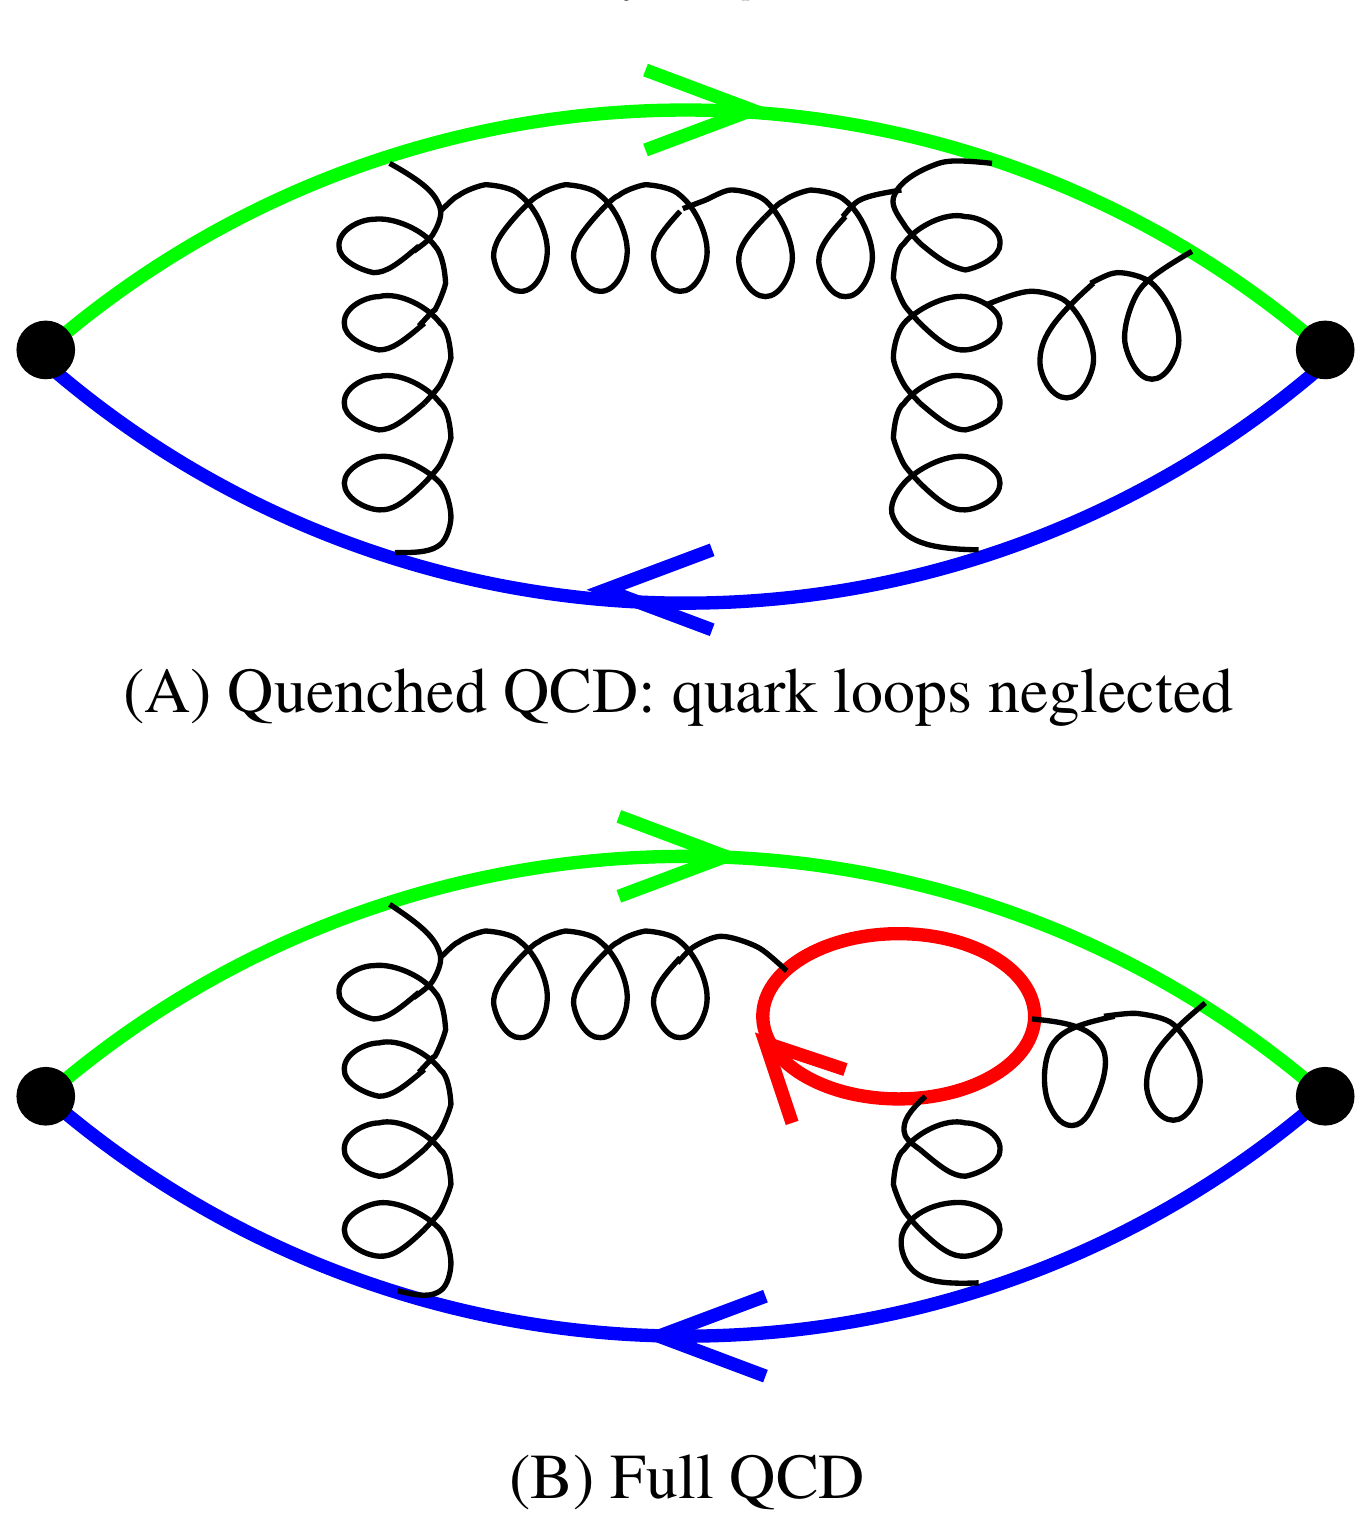
\includegraphics[width=0.8\textwidth]{images/fig16.png}
\caption{An illustration of the difference between quenched QCD and QCD. QQCD has no vacuum polarization loops on virtual gluon lines.}
\label{fig:16}
\end{figure}

Physically, the quenched approximation corresponds to turning off vacuum polarization effects of quark loops. This is illustrated in Fig.~\ref{fig:16} for the pion correlator. One important consequence of neglecting vacuum polarization effects is the behavior of the potential between a $q\bar{q}$ pair as a function of the separation. In the full theory the string breaks by the creation of a $q\bar{q}$ pair out of the vacuum, therefore at large distances there is a screened potential between two mesons. For such screened potential large Wilson loops should show a perimeter law. In QQCD the string does not break and large Wilson loops show an area law. Thus the long distance behavior of the two theories is very different and one might be led to believe that QQCD is a bad approximation. However, because of confinement, the long distance scale that is relevant to hadronic physics has a natural cutoff of a few fermi. Thus, if one can match the potential between some fine scale ($\sim 0.01$ fermi, below which asymptotic freedom makes the calculations perturbative) and the typical size of hadrons ($\sim 1$ fermi) then QQCD could give reasonable estimates for the hadronic spectrum. This argument is really only applicable to heavy onia, where potential models work well. For light quarks one simply has to do the simulations to estimate the size of the distortions. In any case the community has proceeded by assuming that the two theories can be roughly matched by adjusting the quenched coupling constant at some scale like $0.5$ fermi, or equivalently by adjusting the overall scale $\Lambda_{QQCD}$, and hopes that the quenching corrections are small, $10 - 20\%$, for many cases. If this bears out then even QQCD would yield many phenomenologically useful predictions.

In spite of the optimism, the fact remains that QQCD is not a unitary theory, so it is important to understand how it fails. I would like to illustrate its shortcomings with the following examples.

We can calculate the $\rho\pi\pi$ coupling in both QCD and QQCD by measuring the three point function $\langle T[\rho\pi\pi]\rangle$ illustrated in Fig.~\ref{fig:17}A. The difference between the two values is a measure of the validity of QQCD. On the other hand the diagram shown in Fig.~\ref{fig:17}B is absent in QQCD, and the $\rho$ spectral function does not have a cut beginning at $2M_\pi$. Thus, the $\rho\pi\pi$ coupling \textit{cannot} be extracted from an analysis of the $\rho$ 2-point function in QQCD.

\begin{figure}[htbp]
\centering
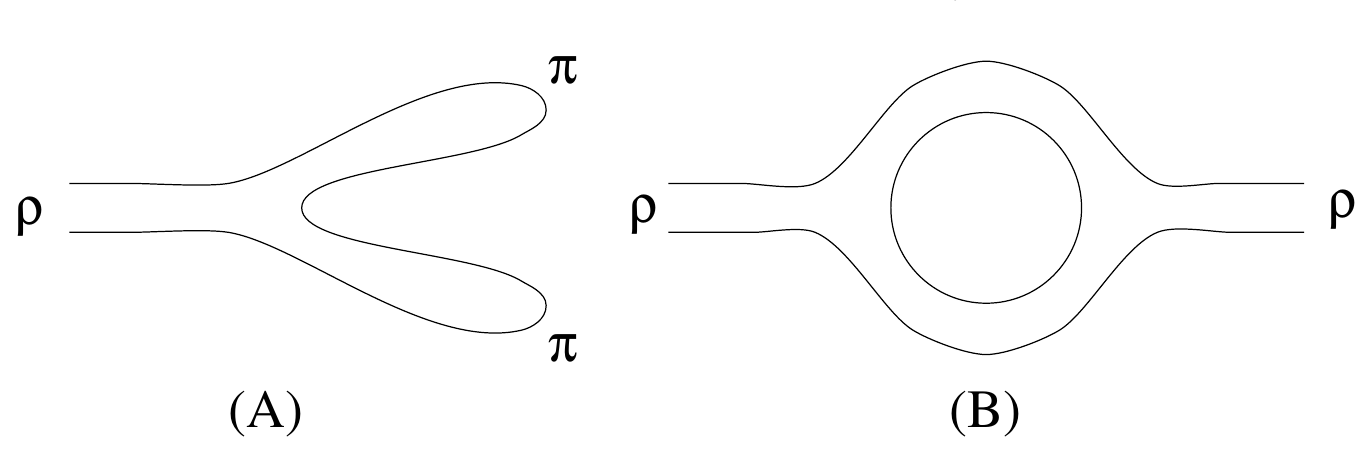
\includegraphics[width=0.8\textwidth]{images/fig17.png}
\caption{The $\rho\pi\pi$ coupling from the $\rho \to \pi\pi$ decay and (B) the $\rho$ correlator in full QCD.}
\label{fig:17}
\end{figure}

A very important difference between full QCD and QQCD is the behavior of the $\eta'$. In full QCD the singlet axial current is anomalous and the $\eta'$ acquires a large mass due to the summation of vacuum polarization graphs shown in Fig.~\ref{fig:18},
\begin{equation}
\frac{1}{p^2 - M^2} + \frac{1}{p^2 - M^2} M_0^2 \frac{1}{p^2 - M^2} + \cdots = \frac{1}{p^2 - M^2 - M_0^2}
\end{equation}
where, for simplicity I have approximated the gluonic coupling by a momentum independent constant $M_0^2$. This is related to the topological susceptibility via the Witten--Veneziano relation $M_0^2 = 2n_f \chi_t / f_\pi^2 = M_{\eta'}^2 + M_\eta^2 - 2M_K^2$ [149]. In QQCD the absence of the vacuum polarization diagrams means that the $\eta'$ propagator has a single and a double pole, i.e.~$(p^2 - M^2)^{-1}$ and the ``hairpin'' term $(p^2 - M^2)^{-1} M_0^2 (p^2 - M^2)^{-1}$, where $M^2$ is the Goldstone pion mass $M_\pi^2$. The fact that the $\eta'$, in the limit $m_q \to 0$ of QQCD, is massless has important consequences. Two groups, Sharpe and collaborators [150], and Bernard and Golterman [151], have investigated these by formulating a chiral perturbation theory for QQCD which retains $\eta'$ as an additional Goldstone boson. I illustrate the differences between $\chi$PT and Q$\chi$PT by considering the behavior of the 2-point correlation function of the pion.

\begin{figure}[htbp]
\centering
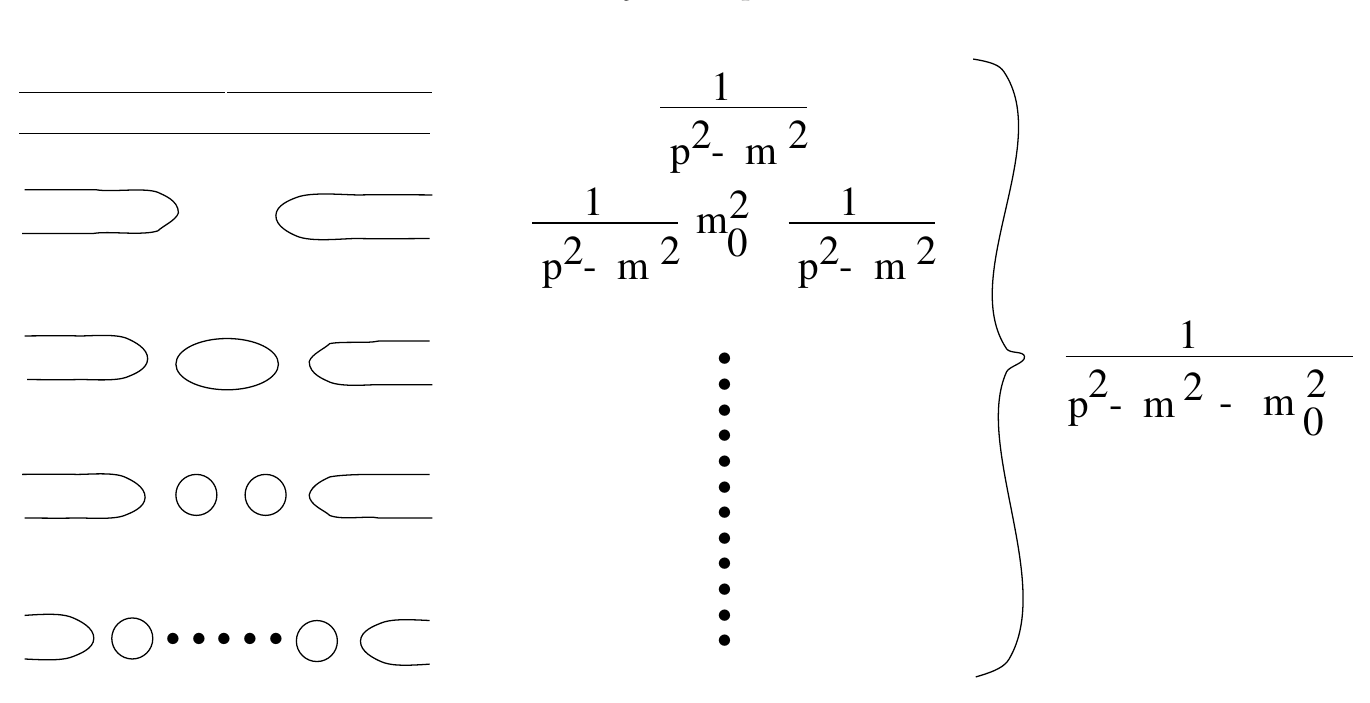
\includegraphics[width=0.8\textwidth]{images/fig18.png}
\caption{The iteration of the $\eta'$ propagator in full QCD. Only the first two diagrams survive in QQCD.}
\label{fig:18}
\end{figure}

\begin{figure}[htbp]
\centering
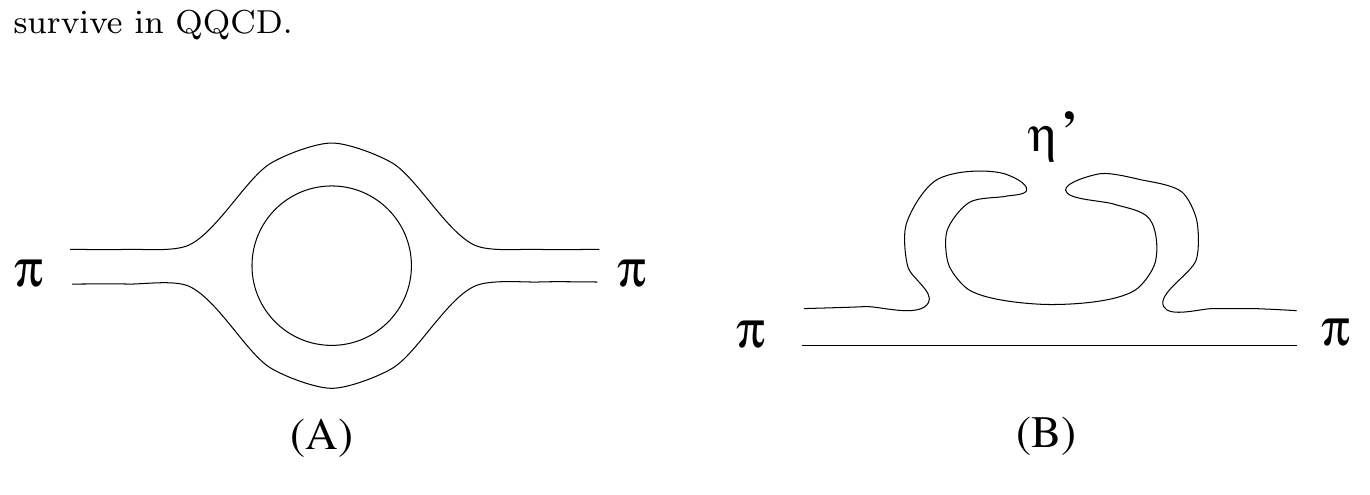
\includegraphics[width=0.8\textwidth]{images/fig19.png}
\caption{The 1-loop correction to the pion propagator in (A) full QCD (B) QQCD.}
\label{fig:19}
\end{figure}

At 1-loop full QCD has the diagram shown in Fig.~\ref{fig:19}A which is absent in QQCD. On the other hand, in QQCD, the hairpin term gives a contribution via the diagram shown in Fig.~\ref{fig:19}B. Such diagrams are neglected in full QCD as they iterate to produce a massive $\eta'$. The chiral expansions for $M_\pi$ and $f_\pi$ in full QCD have been calculated by Gasser and Leutwyler [152],
\begin{equation}
\begin{aligned}
M_\pi^2 &= 2mB\Bigl[1 + X_\pi - \frac{1}{3} X_{\eta_8} + \frac{16}{f_0^2}(2M_K^2 + M_\pi^2)(2L_6 - L_4) \\
&\qquad\qquad + \frac{16}{f_0^2} M_\pi^2 (2L_8 - L_5) + \cdots\Bigr] \\
f_\pi^2 &= f_0\Bigl[1 - 4X_\pi - 2X_K + \frac{16}{f_0^2}(2M_K^2 + M_\pi^2)L_4 + \frac{16}{f_0^2} M_\pi^2 L_5 + \cdots\Bigr]
\end{aligned}
\end{equation}
where $L_i$ are the $O(p^4)$ coefficients, $X_i = M_i^2 \log(M_i^2/\Lambda_{\chi SB}^2)/(4\pi f_0)^2$ are the chiral logs, and $f_\pi = 131$ MeV. In QQCD, Sharpe and Bernard and Golterman [150,151] find that the leading terms are
\begin{equation}
\begin{aligned}
M_\pi^{2Q} &= 2mB_Q\Bigl[1 - \delta \log\frac{M_\pi^2}{\Lambda_{\chi SB}^2} + \cdots\Bigr] \\
f_\pi^Q &= f_Q\Bigl[1 - \frac{16}{f_Q^2} M_\pi^2 \tilde{L}_5 + \cdots\Bigr]
\end{aligned}
\end{equation}
where $\delta = M_0^2 / 24\pi^2 f_\pi^2$ and $\tilde{L}_i$ are the quenched $O(p^4)$ coefficients. The term proportional to $\delta$ is a quenched chiral log and is singular in the limit $m_q = 0$.

The differences, in general, between quenched and unquenched expressions, as illustrated by the above expressions, are
\begin{itemize}
\item All the chiral constants are different in the two theories. For example, $B \neq B_Q$ and $f_0 \neq f_Q$.
\item The normal chiral logs are missing in QQCD.
\item The quenched expressions can be singular in the chiral limit due to the goldstone $\eta'$, i.e.~through terms proportional to $\delta$. These artifacts become dominant as $m_q \to 0$.
\end{itemize}

The first question raised by the analyses of Sharpe and Bernard and Golterman is---are the results of quenched $\chi$PT, an expansion about $m_q = 0$, meaningful if they are singular in that limit? We do not have a formal answer to this question. The approach adopted is to do the simulations and look for such chiral logs by doing fits with and without these terms. The status of this search has been reviewed in [153,154]. The data, while not conclusive, does suggest that $\delta \approx 0.15$, consistent with the value obtained by using phenomenological values for $M_0$ and $f_\pi$.

The second question, assuming that predictions of quenched $\chi$PT make sense, is how does one extract phenomenologically useful results for quantities that require a chiral extrapolation to $\bar{m}$? One approach is to fit the quenched data using the full QCD chiral expansions in a region of quark masses where the quenched artifacts are small. Current data suggest that this region is $m_q \gtrsim m_s/4$. In this case quenching errors are, by definition, a combination of those due to the absence of quark loops and those due to fits being made at heavier quark masses. The second possibility is to fit using the QQCD expression but extrapolate keeping only the terms in the full QCD expressions. This approach has the disadvantage of increasing the number of free parameters. In either case the hope is that there exist quantities for which the QQCD artifacts are small and the differences between QQCD and QCD coefficients are small; in such cases quenched estimates are useful phenomenological predictions. One such example is the $K^0\bar{K}^0$ mixing parameter $B_K$ [155].

In view of these various sources of systematic error, any quantity measured on the lattice depends not only on the input parameters, i.e.~the quark masses and the coupling $\alpha_s$, but also on the lattice size $L$, $a$ (discretization errors are $\propto g^m a^n$ with the powers depending on the order of improvement in the action and operators), the method used to determine the renormalization constants, and the number of dynamical quark flavors $n_f$. While the theoretical understanding of these errors is, in general, not complete, nevertheless, a lot is known and one can make consistency checks on the data. For example, the infinite volume continuum limit results for fixed $n_f$ simulations should be independent of the discretization scheme, the numerical approach used, and the definition of the renormalization constants. As of this writing, results for a number of observables show stability once extrapolated to the $L \to \infty$ and $a \to 0$ limits, albeit in the quenched approximation ($n_f = 0$). We regard this consistency check as the first important step towards providing precise results. Our optimism stems from knowing that for many phenomenologically important quantities ($B_K$, $f_D$, $f_{D_s}$, $f_B$, $f_{B_s}$, $B_B$, $\alpha_s$, and the quark masses) quenched lattice QCD results are already competitive with the best non-lattice methods, and future enhancements in methodology and computer technology will systematically improve their precision.
